% https://es.overleaf.com/latex/templates/project-report/jpzczmpsdzwm

%%% Preamble
\documentclass[paper=leter, fontsize=11pt]{scrartcl}
\usepackage[utf8]{inputenc}
\usepackage[spanish,mexico]{babel}
\usepackage[T1]{fontenc}    % use 8-bit T1 fonts
\usepackage{lmodern}
\usepackage{hyperref}       % hyperlinks
\usepackage{lipsum}
\usepackage[square,numbers]{natbib}

\usepackage[protrusion=true,expansion=true]{microtype}	
\usepackage{amsmath,amsfonts,amsthm} % Math packages
\usepackage[pdftex]{graphicx}	
\usepackage{url}

\usepackage{tikz}

\usepackage{caption}
\usepackage{subcaption}

\graphicspath{ {imgs/} }

\selectlanguage{spanish}
\usepackage[spanish,onelanguage]{algorithm2e}


%%% Custom sectioning
\usepackage{sectsty}
\allsectionsfont{\centering \normalfont\scshape}


%%% Custom headers/footers (fancyhdr package)
\usepackage{fancyhdr}
\pagestyle{fancyplain}
\fancyhead{}											% No page header
\fancyfoot[L]{}											% Empty 
\fancyfoot[C]{}											% Empty
\fancyfoot[R]{\thepage}									% Pagenumbering
\renewcommand{\headrulewidth}{0pt}			% Remove header underlines
\renewcommand{\footrulewidth}{0pt}				% Remove footer underlines
\setlength{\headheight}{13.6pt}


%%% Equation and float numbering
\numberwithin{equation}{section}		% Equationnumbering: section.eq#
\numberwithin{figure}{section}			% Figurenumbering: section.fig#
\numberwithin{table}{section}				% Tablenumbering: section.tab#


%%% Maketitle metadata
\newcommand{\horrule}[1]{\rule{\linewidth}{#1}} 	% Horizontal rule

\title{
		%\vspace{-1in} 	
		\usefont{OT1}{bch}{b}{n}
		\normalfont \normalsize \textsc{Posgrado de Ingeniería de Sistemas} \\ [25pt]
		\horrule{0.5pt} \\[0.4cm]
		\huge Preprocesamiento de datos \\
		\horrule{2pt} \\[0.5cm]
}
\author{
		\normalfont 								\normalsize
        Alberto Benavides\\[-3pt]		\normalsize
        \today
}
\date{}


%%% Begin document
\begin{document}
\maketitle
\section{Sobre los datos}

Se cuenta con un conjunto de datos consistente en históricos de ventas y producción mensuales de entre los años 2014 a 2019 (ambos incluidos) de artículos de la empresa Fritos Totis \cite{totis}. Dicho conjunto de datos se encuentra en formato \texttt{{XLSX}}, propio de los archivos generados por Microsoft Excel \cite{excel}. El acomodo de estos datos está dado en bloques de siete renglones, uno por cada año, por cada artículo definido por un código, con 24 columnas por cada bloque que corresponden, por pares, a los doce meses del año. De cada par de columnas por renglón por artículo, la primera corresponde a la producción y la segunda a la venta. Un ejemplo de esto puede verse en la figura \ref{ejemploExcel} (p. \pageref{ejemploExcel}).

\begin{figure}[t]
    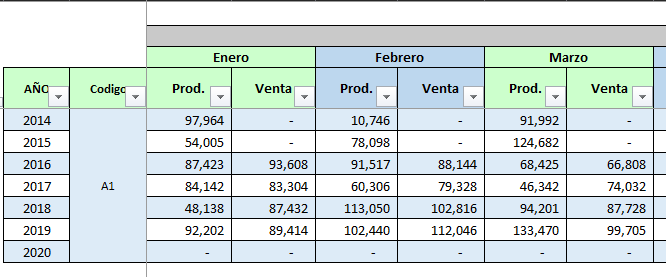
\includegraphics[width=\textwidth]{ejemploExcel}
    \centering
    \caption{Extracto del artículo con código A1 obtenido del documento original en formato \texttt{XLSX}.}
    \label{ejemploExcel}
\end{figure}

\section{Valores separados por comas}

Para poder hacer un análisis de datos es necesario tener un conjunto de los mismos en un formato que facilite su preprocesamiento \cite{preparacion}. Por este motivo, se procede a convertirlos en formato \texttt{CSV} \cite{csv} en renglones que informen, por columnas, el código del artículo, las producciones, ventas y la fecha en que fueron reportadas. Para este fin, se utilizó la librería \texttt{datetime} \cite{datetime} con la que se convirtieron los meses y años a formato de fecha compatible para futuro preprocesamiento de la información. Los datos un ejemplo de los datos procesados se muestra en el cuadro \ref{limpios} (p. \pageref{limpios}). En tal cuadro puede verse que existen valores reportados con el símbolo de \texttt{-} por lo que falta aclarar qué significa dicho símbolo para poder analizar los datos.

\begin{table}[]
	\caption{Ejemplo de datos limpios tras procesamiento.}
	\label{limpios}
	\centering
	\begin{tabular}{c|c|c|c}
    Código & Producción & Ventas & Fecha \\ \hline
    A1 & $97,964$ & - & 2014-01-01 \\
    A1 & $10,746$ & - & 2014-02-01 \\
    A1 & $91,992$ & - & 2014-03-01 \\
    A1 & $50,939$ & - & 2014-04-01 \\
    A1 & $26,826$ & - & 2014-05-01
	\end{tabular}
\end{table}

\raggedright 
\bibliographystyle{plainnat}
\bibliography{../Biblio}

\end{document}